\documentclass{report}
\usepackage{graphicx}
\usepackage{float}
\usepackage[utf8]{inputenc}
\usepackage{amsmath, amsfonts}
\usepackage[a4paper, total={6in, 8in}, textheight=750pt]{geometry}
\graphicspath{ {./images/} }

\title{Project ML2 - 97209 \\ Taming VAE}
\author{David Parnas 337977045 \\ Tamir Shazman 316250877}
\date{}

\DeclareMathOperator{\E}{\mathbb{E}}
\newcommand{\norm}[1]{\left\lVert#1\right\rVert}
\begin{document}
\maketitle


\chapter*{Introduction}
\section*{Latent variable model}
A latent variable model is a statistical model that relates a set of observable variables (so-called manifest variables) to a set of latent variables.
\\ The motivation behind latent variable modeling is to capture complex or conceptual properties of a system that are difficult to quantify or measure directly. For example we can think of a random process that generates millions of pixel-images of dogs. If we want to learn this random process and generate our own images, it will be a difficult task to generate the multitudes of pixels that form these pictures. However, if we think of that random process as the conceptually simpler process of : first choosing a breed of a dog and only after that sampling a picture with the same dog breed, this may lead us to a better model. VAEs strive to create disentangled latent representations that allow choose characteristic such as dog breed. \\ 
Let's denote $X$ as observed data and $z$ as latent variables of the data. \\ Using Bayesian statistics,  we can look at the distribution of z as the prior, and the distribution of $z|X$ as posterior. We assume that the data ($X$) is i.i.d. relative to $P_{data}$. \\ 
Using this modeling, we seek parameters $\theta$ that maximize the log-likelihood of our data:
\begin{gather*}
\theta = \underset{\theta}{\arg\max} \ log \ p_{\theta}(X)=\underset{\theta}{\arg\max} \sum_{i=1}^{n} log \ p_{\theta}(X^{(i)})=\underset{\theta}{\arg\max} \sum_{i=1}^{n}log \int_z p_{\theta}(X^{(i)}|z)p_{Z}(z)dz
\end{gather*}
In most scenarios, the above optimization problem is hard to compute or intractable. To overcome This problem, we can use Monte-Carlo estimator for this integral and just sample from our prior $p_{Z}$ and leading to the following optimization problem: 
\begin{gather*}
\theta = \underset{\theta}{\arg\max} \sum_{i=1}^{n}log \frac{1}{K} \sum_{k=1}^{K} p_{\theta}(X^{(i)}|z_{k}^{(i)})p_{Z}(z_{k}^{(i)}) \quad , when \ z^{k}\sim p_{Z}
\end{gather*}
The main problem with prior sampling as suggested is that is not very informative. If we look at z as a continuous distribution, the sampled z's will most likely to cause $p_{\theta}(X^{(i)}|z^{k})$ to be equal to zero, and thus the $\theta$ parameters that we will get from the problem will not be very informative. \\ That problem lead to the development of importance sampling and the variational inference approach as follows: 
\begin{gather*}
\theta=\underset{\theta}{\arg\max} \sum_{i=1}^{n}log \int_z p_{\theta}(X^{(i)}|z)p_{Z}(z)dz = \underset{\theta}{\arg\max} \sum_{i=1}^{n}log \int_z \frac{q_{\Phi}(z)}{q_{\Phi}(z)}p_{\theta}(X^{(i)}|z)p_{Z}(z)dz= \\ \\ = \underset{\theta}{\arg\max} \sum_{i=1}^{n}log \mathbb{E}_{z \sim q_{\Phi}(z)}[\frac{p_{\theta}(X^{(i)}|z)}{q_{\Phi}(z)}p_{Z}(z)] \approx \underset{\theta}{\arg\max} \sum_{i=1}^{n}log \sum_{k=1}^{K}\frac{p_{\theta}(X^{(i)}|z_{k}^{(i)})}{q_{\Phi}(z_{k}^{(i)})}p_{Z}(z_{k}^{(i)}) \\ \\ , when\ z^{k}\sim q_{\Phi} \ and \ q_{\Phi} \ is \ some \ distribution \ with \ parameters \ \Phi.
\end{gather*}
We can see that a good-informative approximation to $q_{\Phi}(z)$ will be the posterior of z (i.e $z|X^{(i)}$). To achieve a good approximation of $q_{\Phi}(z)$ we'll use KL-diverge and the objective will be: 
\begin{gather*}
\underset{\theta,\Phi}{\arg\max} \sum_{i=1}^{n}log \sum_{k=1}^{K}\frac{p_{\theta}(X^{(i)}|z_{k}^{(i)})}{q_{\Phi}(z_{k}^{(i)})}p_{Z}(z_{k}^{(i)}) - KL(q_{\Phi}(z)||p_{\theta}(z|X))
\end{gather*}
Another derivation to this objection is from Variational Bayesian method.\\
Let us find a good approximation to some posterior\\ \\
\begin{gather*}
KL(q(z)||p(z|X))=\mathbb{E}_{z \sim q(z)}[log \ q(z)-log \ p(z|X)] = \\  
= \mathbb{E}_{z \sim q(z)}[log \ q(z) - log \ \frac{p(z,X)}{p(X)}] = \\ 
=(1) \mathbb{E}_{z \sim q(z)}[log \ q(z) - log \ p(z) - log \ p(X|z)] + log \ p(X) \\ 
\end{gather*}
According to (1), if we want to maximize the log-likelihood we need to maximize : \\ \\
$log \ p(X) = \underbrace{\mathbb{E}_{z \sim q(z)}[-log \ q(z) + log \ p(z) + log \ p(X|z)]}_{ELBO}+KL(q(z)||p(z|X))$ \\ \\
The Evidence lower bound (ELBO) approximately lower bounds the above term because KL is always positive. Thereby, the following inequality: \\ \\
$log \ p(X) = \underbrace{\mathbb{E}_{z \sim q(z)}[-log \ q(z) + log \ p(z) + log \ p(X|z)]}_{ELBO}+KL(q(z)||p(z|X)) \underbrace{\geq}_{KL \geq 0} ELBO $ \\
\section*{ELBO Maximization}
We maximize ELBO and not ($\mathbb{E}_{z \sim q_{\Phi}(z)}[-log \ q_{\Phi}(z) + log \ p(z) + log \ p_{\theta}(X|z)]+KL(q_{\Phi}(z)||p(z|X))$) because we do not know the posterior. However, we can see that given X, the log-likelihood is not dependent on $q_{\Phi}(z)$ and because ELBO lower bounds the above term, maximizing ELBO is equivalent to minimizing the KL-term.\\
Therefore, our final optimization problem is: 
\begin{gather*}
\underset{\theta, \Phi}{\arg\max} \mathbb{E}_{z \sim q_{\Phi}(z)}[-log \ q_{\Phi}(z) + log \ p(z) + log \ p_{\theta}(X|z)] \approx \underset{\theta, \Phi}{\arg\max} \sum_{i=1}^{n}log \sum_{k=1}^{K}\frac{p_{\theta}(X^{(i)}|z_{k}^{(i)})}{q_{\Phi}(z_{k}^{(i)})}p_{Z}(z_{k}^{(i)})\\
\end{gather*}
\section*{ELBO Maximization via Neural Network (Variational Auto Encoder and Amortized Inference)}
When trying to solve the ELBO Maximization problem, we first need to choose a family of distribution $F$ with parameters $\Phi$ for $q(z)$. Most of the time the normal distribution is used. Then we wish to solve : 
\begin{gather*}
\underset{\theta, \Phi}{\arg\max} \ \mathbb{E}_{X\sim data}[\mathbb{E}_{z \sim q_{\Phi}(z)}[-log \ q_{\Phi}(z) + log \ p(z) + log \ p_{\theta}(X|z)]] \approx \\
\approx \underset{\theta, \Phi}{\arg\max} \frac{1}{n}\sum_{i=1}^{n}log \sum_{k=1}^{K}\frac{p_{\theta}(X^{(i)}|z_{k}^{(i)})}{q_{\Phi}(z_{k}^{(i)})}p_{Z}(z_{k}^{(i)})
\end{gather*}
This can be a hard problem to solve,and every group of $X$ requires a solution. This is unfeasible and prevents generalization. Instead of optimizing a set of free parameters for each x, we optimized a parameterized function that maps from the observation space, $X$, to the parameters of the approximate posterior distribution.\\
This is known as amortized inference. \\
In practice, we use neural networks that receive observations as input, and outputs the mean and variance parameters for the latent variable associated with that observation. We can then optimize the parameters of this neural network instead of the individual parameters of each observation, allowing for generalization.
\begin{figure}[t]
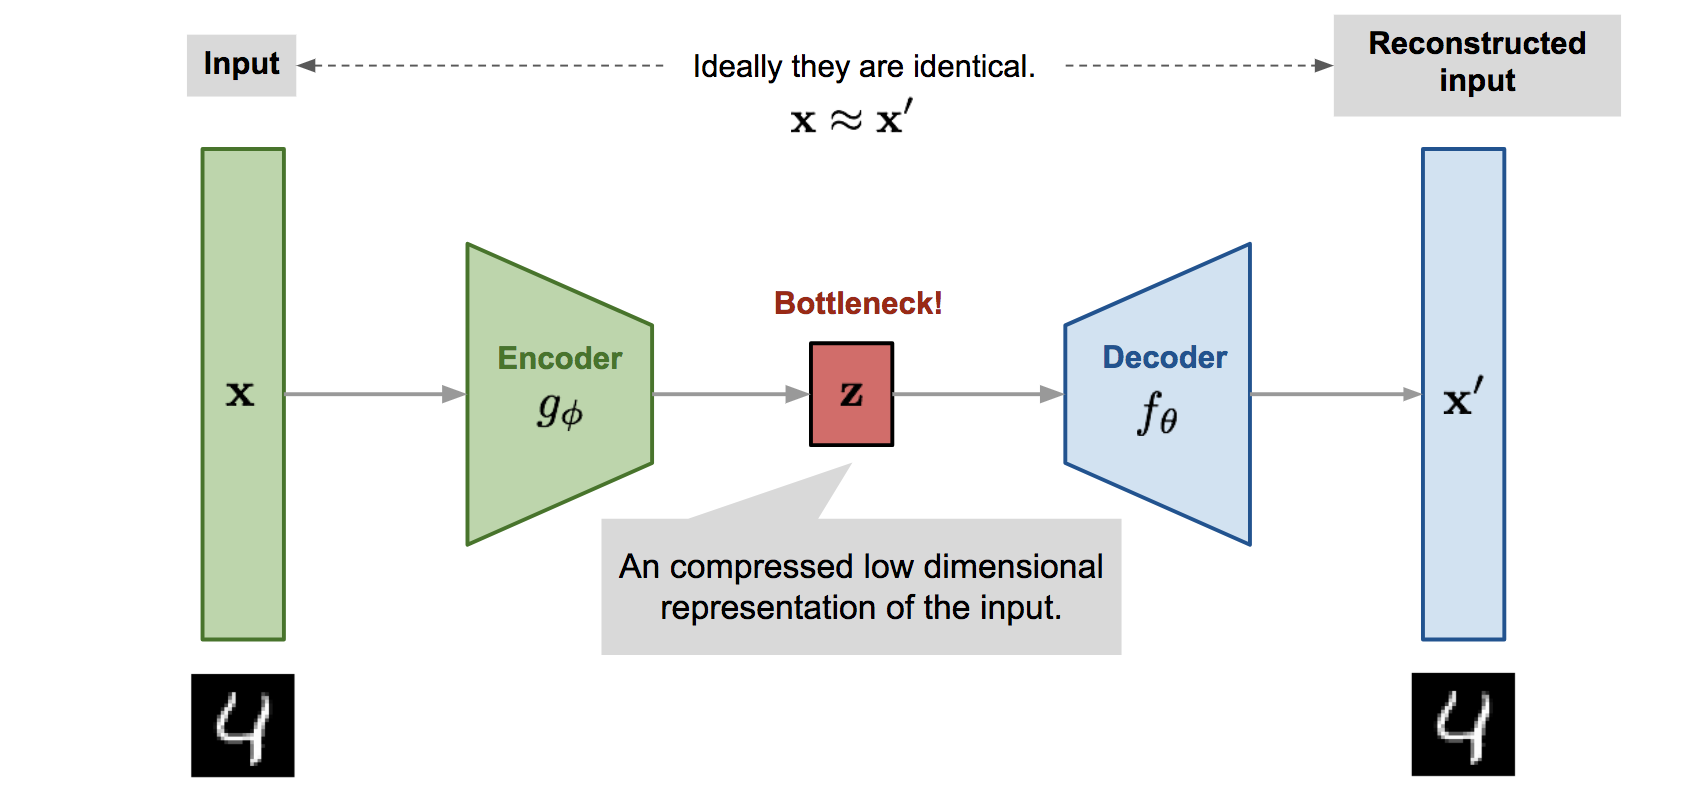
\includegraphics[width=\textwidth]{autoencoder-architecture}
\caption{We can think of this as a encoder (maximize by $\Phi$) and a decoder (maximize by $\theta$)}
\centering
\end{figure}
\\ \\ \\ \\ \\ \\ \\
We can look at the ELBO objective in another interesting way.\\
Let rewrite it to another formation :
\begin{gather*}
ELBO=\mathbb{E}_{z \sim q_{\Phi}(z)}[-log \ q_{\Phi}(z) + log \ p(z) + log \ p_{\theta}(X|z)] = \\ \\
= \underbrace{\mathbb{E}_{z \sim q_{\Phi}(z)}[log \ p_{\theta}(X|z)]}_{Reconstruction loss} - \underbrace{KL(q_{\Phi}(z|X)||p(z))}_{Regularization}
\end{gather*}
The reconstruction term assures that the model reconstructs $X$ accurately-how close is the input to the output. The regularization term adds regularization to the model preventing the NN model from overfitting the training data.\\
In order to prevent this, the regularization term keeps the distribution of the posterior simple. \\ \\

\section*{Optimization and representation trick}
The optimization problem that we saw above may be written:
\begin{gather*}
\underset{\theta, \Phi}{\arg\max} \ \mathbb{E}_{z \sim q_{\Phi}(z)}[f(z;\theta)] = \underset{\theta, \Phi}{\arg\max} \int_{z} q_{\Phi}(z)f(z;\theta)dz
\end{gather*}
Solving this problem requires the use of SGD or GD methods, which in turn need the derivatives. To find the derivatives we need to compute the integral, which are often hard to solve or intractable. We have seen that we can estimate the integral using Monte-Carlo approximation. However, using the Monte-Carlo approximation, removes the integrals dependency on $\Phi$ and thus we cannot find the derivative w.r.t $\Phi$ \\
To solve that we can rearrange the derivative w.r.t $\Phi$ :
\begin{gather*}
\nabla_{\Phi} (\mathbb{E}_{z \sim q_{\Phi}(z)}[f(z;\theta)]) =  \int_{z} \nabla_{\Phi}(q_{\Phi}(z))f(z;\theta)dz = \int_{z} \frac{q_{\Phi}(z)}{q_{\Phi}(z)}\nabla_{\Phi}(q_{\Phi}(z))f(z;\theta)dz = \\
= \int_{z} q_{\Phi}(z)\nabla_{\Phi}(log \ q_{\Phi}(z))f(z;\theta)dz = \mathbb{E}_{z \sim q_{\Phi}(z)}[\nabla_{\Phi}(log \ q_{\Phi}(z))f(z;\theta)] \approx \\ \approx \frac{1}{K}\sum_{k=1}^{K}\nabla_{\Phi}(log \ q_{\Phi}(z^{(k)})f(z;\theta)
\end{gather*}
This solves the above problem, but it turns out that this approximation is very noisy and requires many samples from $q_{\Phi}$. \\
To overcome this issue we can use the reparametrization trick : we choose $q_{\Phi} \sim N(\mu, \sigma^2)$ and then we using the normal distribution properties :
\begin{gather*}
\mathbb{E}_{z \sim q_{\Phi}(z)}[f(z;\theta)] = \mathbb{E}_{\epsilon \sim N(0,I)}[f(\mu_{\Phi} + \sigma_{\Phi}\epsilon;\theta)] \approx \frac{1}{K}\sum_{k=1}^{K}f(\mu_{\Phi} + \sigma_{\Phi}\epsilon^{(k)};\theta), \\ when \ \epsilon^{(k)} \sim N(0,I)
\end{gather*} 
Now to find an estimation for the derivative w.r.t $\Phi$. The parameters $\Phi$ are $\mu_{\Phi}, \ \sigma^2_{\Phi}$.
\begin{figure}[H]
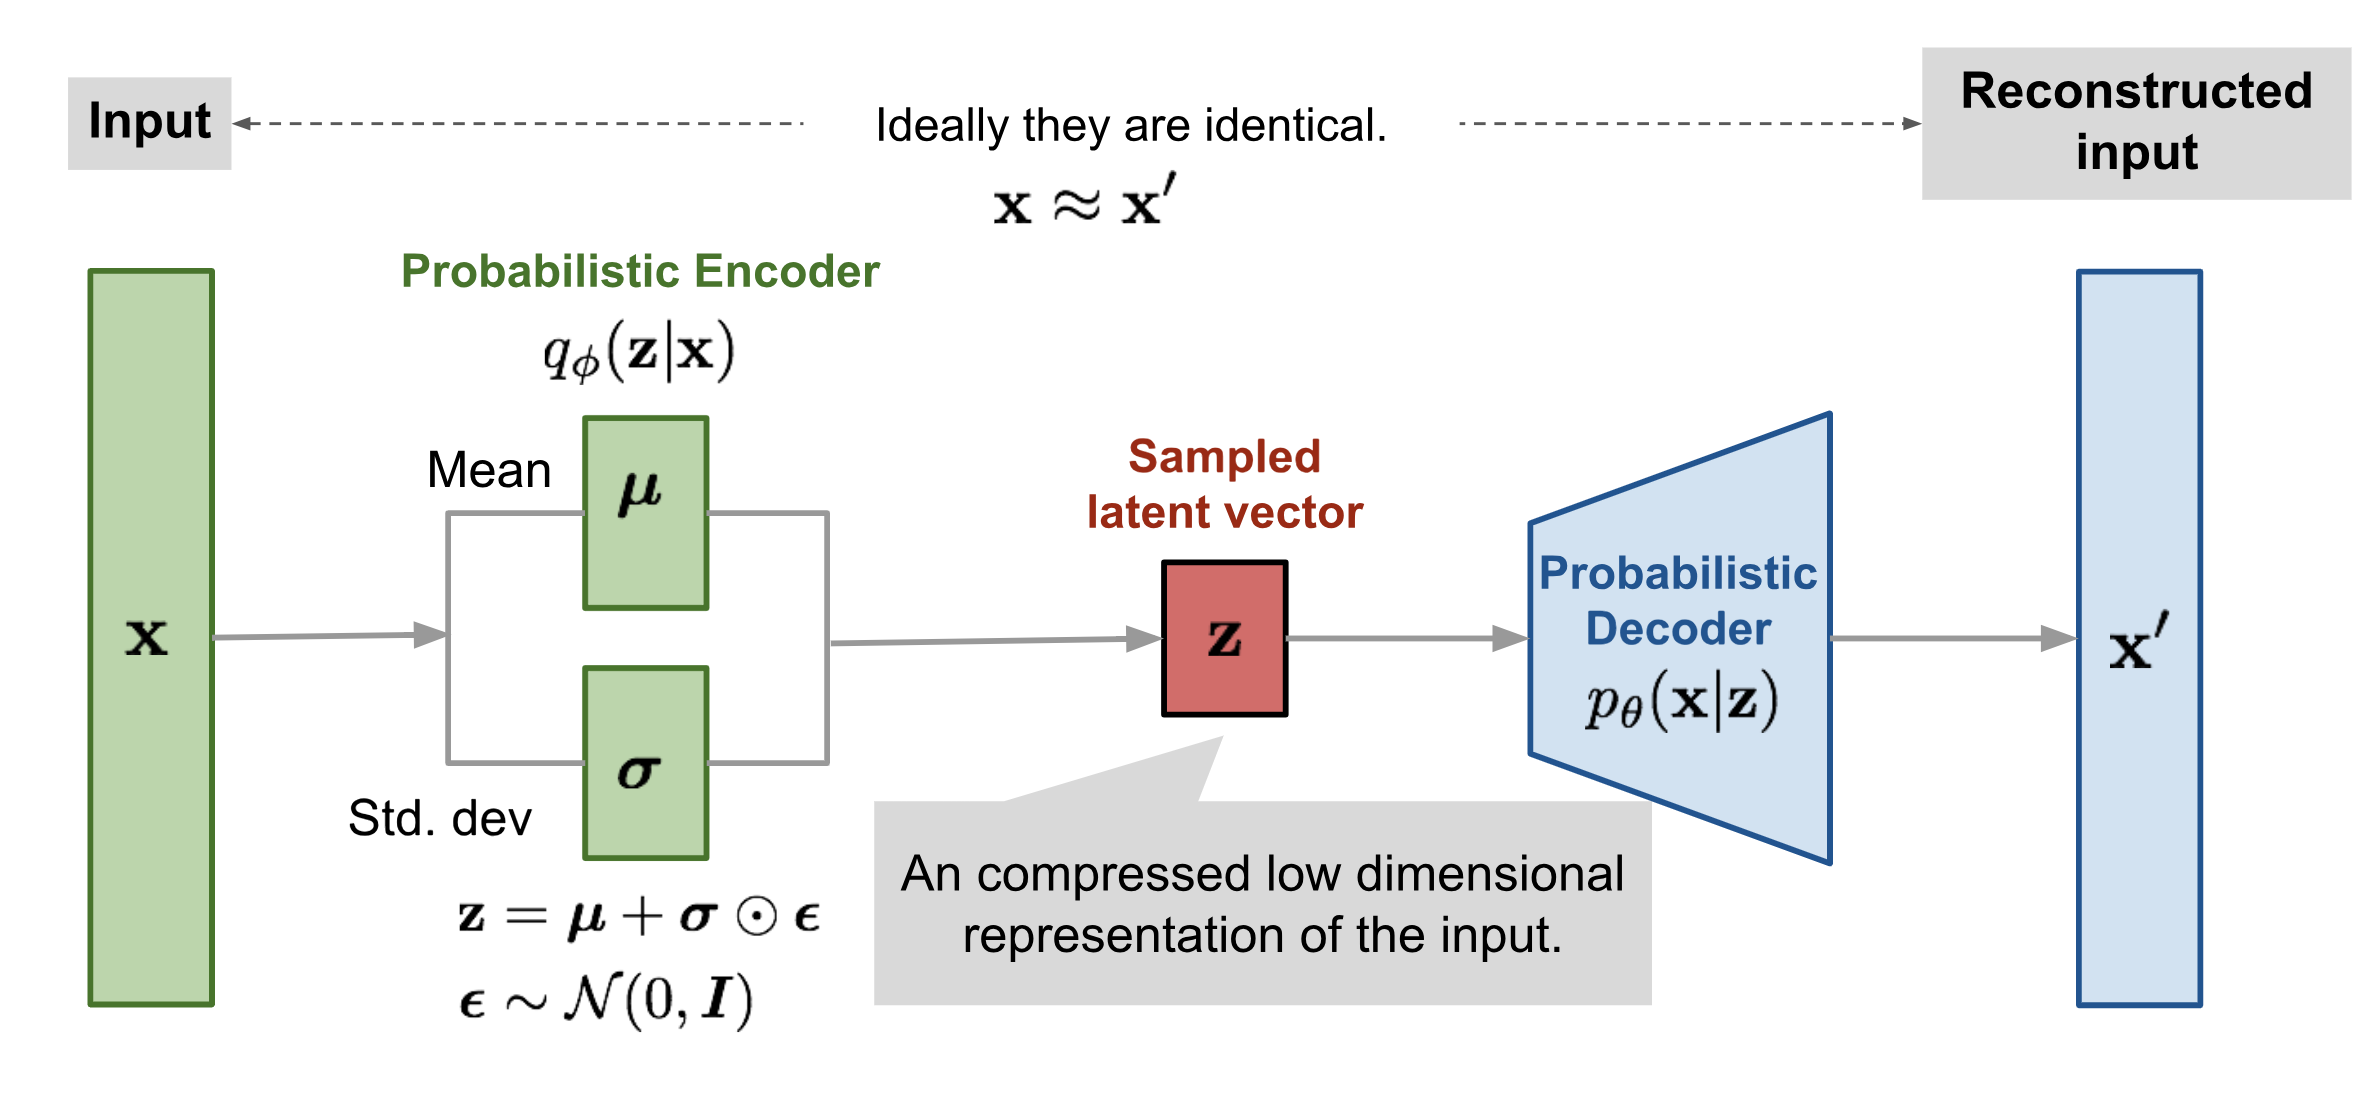
\includegraphics[width=\textwidth]{vae-gaussian}
\caption{To use the representation trick we just need to let $q_{\Phi}\sim N(0,I)$ and find an approximation to the derivative w.r.t $\Phi$ just by sample from the standard Gaussian}
\centering
\end{figure}

\chapter*{Quick Overview}
The papers main goals are:
\begin{enumerate}
\item Offer a deeper understanding of common problems with VAEs
\item Discuss the relationship between the prior and marginal posterior of the latent space
\item Relate VAEs to other fields-Spectral Clustering and Statistical Mechanics
\item GECO - a principled approach to managing the importance given to reconstruction error versus the KL term during training
\end{enumerate}

\section*{1. Common problems with VAEs}
There are two primary problems that affect the generation of random samples with VAEs. The first is "holes"-provided with a sample point in the latent space the decoder fails to construct a meaningful data point in the observed space. The most intuitive example of this is a VAE trained on pictures. A hole occurs when a sampled point is decoded as an almost totally black picture. There is a "hole" in the latent space resulting in an empty picture being reconstructed.
The second common problem is blurred reconstruction. Unlike a "hole," the VAE succeeds in constructing a meaningful data point in the observed space. Returning to the earlier example, the picture is not black. It is, however, blurry. The literature has often attributed this phenomena to the use of Gaussian posteriers. However, the authors claim that blurred reconstruction occurs as a result of the latent sample being found in the cross section of the "domains"/support of several decoders. \\
\section*{2. The relationship between the prior and marginal posterior of the latent space}
The authors continue building a deeper understanding of VAEs behavior. They show that after making certain assumptions about the decoders, it can be shown that the marginal posterior equals the prior.
\section*{3. Relating VAEs to other fields}
Here the authors waste our and everyone's time by pretending to prove certain intuitions that they seem to have felt would make their paper more interesting. Like their "proofs" in this part of the paper, they were wrong.
\section*{4. GECO}
Having expanded the theory on current VAEs, the authors offer the GECO algorithm. GECO offers a more general optimization problem and a method for controlling the trade-off between the reconstruction error and the KL term during training.\\
Instead of ELBO:
\begin{gather*}
{ELBO} =  \E_{\rho(x)}\left[[\E_{q(z|x)}[\ln{p(x|z)}] - KL[q(z|x) \| \pi(z)]\right]
\end{gather*}
GECO uses:
\begin{gather*}
L_{\lambda} = \E_{\rho(x)}\left[KL[q(z|x) \| \pi(z)] + \lambda^{T}\E_{q(z|x)}[\mathcal{C}(x, g(z))\right]
\end{gather*}
Although both contain a term controlling the reconstruction error and the KL divergence, GECO changes two things. 1. It allows for a variety of reconstruction error constraints, generalized as $\mathcal{C}(x, g(z))$. 2. Similar to $\beta$-VAEs it formulates the reconstruction error as a Lagrangian constraint with a Lagrangian multiplier.\\
The paper "beta-VAE: Learning Basic Visual Concepts with a Constrained Variational Framework" shows improved results on ELBO by formulating the reconstruction error as a Lagrangian constraint with a Lagrangian multiplier. This allows for the trade-off between the reconstruction error and KL divergence to be controlled by $\beta$, the Lagrangian multiplier. This gives the ML practitioner more customizability in the $\beta$-VAE model relative to the simple VAE model. However, it adds a hyperparameter that must be found.\\
The authors offer the GECO algorithm using the above optimization problem and, critically, a method for adjusting the Lagrangian multiplier during training. They claim that this prevents "over optimizing" the reconstruction error at the expense of the KL term, resulting in a non-optimal latent distribution space.

\section*{}
We summarize these ideas in more detail below with proofs.

\chapter*{Understanding Holes and Blurred Reconstructions}
The authors show that the optimal decoder, g(z), is a convex linear combination of the training data weighted by the encoders, $q(z|x)$.
As a result, when $q(z|x)\approx 0$ there is a "hole" in the decoder and that blurring occurs when there is overlap between the supports of multiple $x$'s decoders, $q(z|x)$.\\
In order to do so, they use the stationary points of ELBO.

\section*{Stationary Points Using ELBO}
\begin{gather*}
{ELBO} =  \E_{\rho(x)}\left[[\E_{q(z|x)}[\ln{p(x|z)}] - KL[q(z|x) \| \pi(z)]\right]
\end{gather*}

We will further develop the expression using the assumptions that the authors make in their derivations.

\raggedright
They make the following assumptions:\par

\centering
$\rho(x) = \frac{1}{n} \sum_{i=1}^{n}\delta^*(x-x_i)$

$\pi(z) = \mathcal{N}(\textbf{0}, \mathcal{I})$

$p(x|z) = \mathcal{N}(g(z), \sigma^2)$
\par

\raggedright
*$\delta$ represents the Dirac measure.
\par

\begin{gather*}
{ELBO} =  \E_{\rho(x)}\left[[\E_{q(z|x)}[\ln{p(x|z)}] - KL[q(z|x) \| \pi(z)]\right]
\approx \sum_{x}\rho(x)\left(\sum_{z} q(z|x) \ln{p(x|z)} - \sum_{z} ln \frac{q(z|x)}{\pi(z)}\right)
\end{gather*}

By the definition of Dirac measure, $\forall x,$  $\rho(x) = \frac{\mathcal{I}_{(x=x_i)}}{n}$
Therefore, we receive the following:
\begin{gather*}
\frac{1}{n}\sum_{x}\sum_{z} q(z|x) \ln{p(x|z)} - \sum_{z} ln \frac{q(z|x)}{\pi(z)}
\end{gather*}
\par

We will now find the partial derivatives of the ELBO function by decoder, $g(z)$, and encoder, $q(z|x)$.
\par

\subsection*{Decoder}
\begin{equation}
\frac{\partial}{\partial g(z)}\frac{1}{n}\sum_{x}\sum_{z} q(z|x) \ln{p(x|z)} - ln \frac{q(z|x)}{\pi(z)}
\end{equation}
We will plug in the distribution for $p(x|z) = \mathcal{N}(g(z), \sigma^2)$
\begin{equation}
\frac{\partial}{\partial g(z)}\frac{1}{n}\sum_{x}\sum_{z} q(z|x) \ln{\frac{1}{\sqrt[]{2\pi\sigma^2}}}e^{-\frac{\norm{x-g(z)}^2}{2\sigma^2}} - \ln\frac{q(z|x)}{\pi(z)}
\end{equation}
\begin{equation}
\frac{\partial}{\partial g(z)}\frac{1}{n}\sum_{x}\sum_{z} q(z|x) \ln{\frac{1}{\sqrt[]{2\pi\sigma^2}}}-\frac{\norm{x-g(z)}^2}{2\sigma^2} - \ln\frac{q(z|x)}{\pi(z)}
\end{equation}
\begin{equation}
\frac{1}{n}\sum_{x}-\frac{q(z|x)(x-g(z)}{\sigma^2}
\end{equation}
Therefore, setting the partial derivative to zero to find the stationary point, we find the following relationship between decoder and encoders:
\begin{gather*}
g(z) = \frac{\sum_{x}{q(z|x) x}}{\sum_{x}{q(z|x)}}
\end{gather*}
Thus the decoder is a convex linear combination of the training data weighted by the encoders, $q(z|x)$.
\par

\subsection*{Encoder}
\setcounter{equation}{0}
\begin{equation}
\frac{\partial}{\partial q(z|x)}\frac{1}{n}\sum_{x}\sum_{z} q(z|x) \ln{p(x|z)} - ln \frac{q(z|x)}{\pi(z)}
\end{equation}
\begin{equation}
\frac{1}{n}\left[{\ln{\frac{1}{\sqrt[]{2\pi\sigma^2}}}-\frac{\norm{x-g(z)}^2}{2\sigma^2} + \ln{\frac{q(z|x)}{\pi(z)} + 1}}\right]
\end{equation}
The paper only shows a proportional relationship, ignoring the constants. The simplified equation is:
\begin{equation}
-\frac{\norm{x-g(z)}^2}{2\sigma^2} + \ln{\frac{q(z|x)}{\pi(z)}}
\end{equation}
Therefore, setting the partial derivative to zero to find the stationary point, we find the following relationship between encoder and decoder:
\begin{gather*}
q(z|x) \propto \pi(z)e^\frac{-\norm{x-g(z)}^2}{2\sigma^2}
\end{gather*}

\section*{Holes}
Having seen that $g(z) = \frac{\sum_{x}{q(z|x) x}}{\sum_{x}{q(z|x)}}$, it easy to see that if $\forall x, q(z|x) \approx 0$ then also $g(z) \approx 0$ resulting in holes.

\section*{Blurred Reconstructions}
The authors claim that blurred reconstruction is not primarily caused by using Gaussian models in the likelihood. Rather, it is from overlap in the support of multiple $q(z|x_{i})$.
\par
They show there results by replacing $q(z|x_{i})$ with $\frac{\pi(z)\mathcal{I}(z\in\Omega_{i})}{\pi_{i}}$ s.t. $\pi_{i} = \E_{\pi(z)}[\mathcal{I}(z\in\Omega_{i}]$
Therefore,
\setcounter{equation}{0} 
\begin{equation}
g(z) = \sum_{i}x_{i}\frac{q(z|x_{i})}{\sum_{j}q(z|x_{j})}
\end{equation}
Because $\pi(z)$ appears in the numerator and denominator it is canceled out and we get
\begin{equation}
\sum_{i}x_{i}\frac{\frac{\mathcal{I}(z\in\Omega_{i})}{\pi_{i}}}{\sum_{j}\frac{\mathcal{I}(z\in\Omega_{j})}{\pi_{j}}}
\end{equation}
As we can see, when z is uniquely found within the support of a specific $x_i$ then we get:
\begin{gather*}
\sum_{i}x_{i}\frac{\frac{\mathcal{I}(z\in\Omega_{i})}{\pi_{i}}}{\sum_{j}\frac{\mathcal{I}(z\in\Omega_{j})}{\pi_{j}}} = x_{i}\frac{\frac{1}{\pi_{i}}}{\frac{1}{\pi_{i}}} = x_{i}
\end{gather*}
However, if z is found in the support of multiple x then g(z) is a weighted average of these x's, resulting in blurred reconstructions.

\section*{Conclusion}
In conclusion, the authors use the stationary point $g(z) = \frac{\sum_{x}{q(z|x) x}}{\sum_{x}{q(z|x)}}$ in order to show that "holes" occur when $q(z|x) \approx 0$. They also show that the decoder $g(z)$ is a linear combination of $q(z|x)$. Therefore, when a z is part of the support of multiple $q(z|x)$, it is reconstructed as a blurry, weighted average of the respective x.

\chapter*{Relationship of Optimal Encoders to the Prior}
The authors claim that when the encoders $q(z|x_{i}) = \frac{\pi(z)\mathcal{I}({z\in\Omega_{i}})}{\pi_{i}}$ s.t. $\pi_{i} = \E_{\pi(z)}[\mathcal{I}(z\in\Omega_{i}]$, they are fixed points and, when optimized, form an equiprobable partition of the latent probability space. This in turn results in the marginal posterior being equal to the prior.

\section*{Proving Fixed Points}
Before we can show that $q(z|x)$ are fixed points, we must show that $\sigma^{2}$ approaches zero as the encoders and decoders are optimized.\\

\subsection*{1. $\sigma^2$ approaches zero}
\setcounter{equation}{0}
\begin{equation}
{ELBO} =  \E_{\rho(x)}\left[[\E_{q(z|x)}[\ln{p(x|z)}] - KL[q(z|x) \| \pi(z)]\right]
= \sum_{x}\rho(x)\left(\sum_{z} q(z|x) \ln{p(x|z)} - \sum_{z} ln \frac{q(z|x)}{\pi(z)}\right)
\end{equation}
We will note that the KL term is not dependent on $\sigma^2$. Therefore, we will ignore it as it will become zero in the partial derivative.
\begin{equation}
\frac{\partial}{\partial \sigma^2}\E_{\rho(x)q(z|x)}-\frac{1}{2}\left[\ln{2\pi}-\ln{\sigma^2}-\frac{\norm{x-g(z)}^2}{\sigma^2}\right]
\end{equation}
\begin{equation}
\E_{\rho(x)q(z|x)}\left[-\frac{1}{2}\left(-\frac{1}{\sigma^2}+\frac{\norm{x-g(z)}^2}{(\sigma^2)^2}\right)\right] 
\end{equation}
Setting the partial derivative to zero and noticing that $\sigma^{2}$ is not a random variable related to the expectation, we find:
\begin{equation}
\sigma^{2} = \E_{\rho(x)q(z|x)}\left[\norm{x-g(z)}^{2}\right]
\end{equation}

Therefore, as optimization brings g(z) closer to x, $\sigma^2$ approaches zero.

\subsection*{2. Simplifying g(z)}
As we saw earlier, $g(z)=\frac{\sum_{x}{q(z|x) x}}{\sum_{x}{q(z|x)}}$

We also previously mentioned that in their proofs the authors replace $q(z|x_{i})$ with $\frac{\pi(z)\mathcal{I}({z\in\Omega_{i}})}{\pi_{i}}$ s.t. $\pi_{i} = \E_{\pi(z)}[\mathcal{I}(z\in\Omega_{i})]$\\
Let us note that assuming that $\lbrace{{\Omega_i}\rbrace}_{i=1}^n$ forms a partition of the latent probability space then:

\begin{gather*}
\forall x_i, \frac{q(z|x_i)}{\sum_j q(z|x_j)} = \frac{\frac{\pi(z)\mathcal{I}({z\in\Omega_{i}})}{\pi_{i}}}{\sum_j \frac{\pi(z)\mathcal{I}({z\in\Omega_{j}})}{\pi_{j}}} = \frac{\frac{\pi(z)\mathcal{I}({z\in\Omega_{i}})}{\pi_{i}}}{\frac{\pi(z)\mathcal{I}({z\in\Omega_{i}})}{\pi_{i}}} = \mathcal{I}(z\in\Omega_i)
\end{gather*}

Therefore,
\begin{gather*}
g(z)=\frac{\sum_{i}{q(z|x_i) x_i}}{\sum_{i}{q(z|x_i)}} = \sum_i \mathcal{I}(z\in\Omega_i)x_i
\end{gather*}

\subsection*{3. $q(z|x)$ are fixed points}
Now we can continue to show that $q(z|x)$ are fixed points.\\

\begin{gather*}
q(z|x) \propto \pi(z)e^\frac{-\norm{x-g(z)}^2}{2\sigma^2}
\end{gather*}

Combining these equations and dividing by the necessary constant, we get:
\setcounter{equation}{0}
\begin{equation}
q(z|x_i) = \lim_{\sigma^2\to0}\frac{\pi(z)e^\frac{-\norm{x_i-g(z)}^2}{2\sigma^2}}{\sum_z\pi(z)e^\frac{-\norm{x_i-g(z)}^2}{2\sigma^2}}
\end{equation}
\begin{equation}
q(z|x_i) = \lim_{\sigma^2\to0}\frac{\pi(z)\sum_k e^\frac{-\norm{x_i- x_k}^2}{2\sigma^2}\mathcal{I}(z\in\Omega_k)}{\sum_z\pi(z)\sum_j e^\frac{-\norm{x_i- x_j}^2}{2\sigma^2}\mathcal{I}(z\in\Omega_j)}
\end{equation}
\begin{equation}
q(z|x_i) = \frac{\pi(z)\mathcal{I}(z\in\Omega_i)}{\pi_i}
\end{equation}
And this is a fixed-point for any prior $\pi(z)$ constrained by a partition such as $\lbrace{{\Omega_i}\rbrace}_{i=1}^n$

\section*{Proving Equiprobable Partition of the latent probability space}
Plugging these fixed points into the KL term we get:
\setcounter{equation}{0}
\begin{equation}
KL = \E_{\rho(x)q(z|x)}\left[\ln{\frac{q(z|x)}{\pi(z)}}\right] = \frac{1}{n} \sum_i \sum_z \frac{\pi(z)\mathcal{I}({z\in\Omega_{i}})}{\pi_{i}}\ln{\frac{\pi(z)\mathcal{I}(z\in\Omega_i)}{\pi(z)*\pi_i}}
\end{equation}
\begin{equation}
= \frac{1}{n} \sum_i \sum_z \frac{\pi(z)\mathcal{I}({z\in\Omega_{i}})}{\sum_z \pi(z)\mathcal{I}(z\in\Omega_i)}\ln{\frac{\pi(z)\mathcal{I}(z\in\Omega_i)}{\pi(z)*\pi_i}}
\end{equation}
\begin{equation}
= \frac{1}{n} \sum_i \sum_z \frac{\mathcal{I}({z\in\Omega_{i}})}{\sum_z \mathcal{I}(z\in\Omega_i)}\ln{\frac{\mathcal{I}(z\in\Omega_i)}{\pi_i}}
\end{equation}
\begin{equation}
= \frac{1}{n} \sum_i \ln{\frac{1}{\pi_i}} = -\frac{1}{n} \sum_i \ln{\pi_i}
\end{equation}
Solving for the maximal values of $\pi_i$ using the Lagrangian with the usual constraints that assume that $\pi_i$ a probability, we find:
\begin{equation}
-\frac{1}{n}\sum_i\ln{\pi_i} +\eta(\sum_i\pi_i-1)-\sum_i\lambda_i^1\pi_i +\sum_i\lambda_i^2(\pi_i-1)
\end{equation}
For some $i$
\begin{equation}
\frac{\partial}{\partial \pi_i}\left(-\frac{1}{n}\sum_i\ln{\pi_i} +\eta(\sum_i\pi_i-1)-\sum_i\lambda_i^1\pi_i +\sum_i\lambda_i^2(\pi_i-1)\right)= \frac{1}{n*\pi_i} + \eta - \lambda_i^1 + \lambda_i^2
\end{equation}
When setting the partial derivative to zero and assuming that $\pi_i \neq 0$ or $1$ we get
\begin{equation}
\frac{1}{n*\eta} = \pi_i
\end{equation}
Using the condition that $\sum_i\pi_i=1$,
\begin{equation}
\sum_i\frac{1}{n*\eta} = \sum_i\pi_i
\end{equation}
\begin{equation}
\frac{1}{\eta} = 1
\end{equation}
Therefore, $\eta = 1$ and $\forall i, \pi_i = \frac{1}{n}$

We remind the reader that $\pi_{i} = \E_{\pi(z)}[\mathcal{I}(z\in\Omega_{i})]$, which is to say the proportion of z in $\Omega_i$. Therefore, if $\forall i, \pi_i = \frac{1}{n}$ then the z are equally distributed between the partition $\lbrace{{\Omega_i}\rbrace}_{i=1}^n$.

\section*{Marginal Posterior Equal to Prior}
In light of the previous mathematical developments, we look at the marginal posterior $q(z)$ given a partition $\lbrace{{\Omega_i}\rbrace}_{i=1}^n$.
\begin{gather*}
g(z) = \frac{1}{n}\sum_i q(z|x_i) = \frac{1}{n}\sum_i \frac{\pi(z)\mathcal{I}(z\in\Omega_i)}{\pi_i} = \frac{n * \pi(z)}{n} \sum_i \mathcal{I}(z\in\Omega_i)= \pi(z)
\end{gather*}
Therefore, optimal solutions for VAE's encoders are inference models that cover the latent space in such a way that their marginal is equal to the prior.

\section*{Conclusion}
The authors show that $q(z|x_{i}) = \frac{\pi(z)\mathcal{I}({z\in\Omega_{i}})}{\pi_{i}}$ s.t. $\pi_{i} = \E_{\pi(z)}[\mathcal{I}(z\in\Omega_{i})]$ are fixed points and upon convergence to these fixed points, ELBO is maximized when the marginal posterior equals the prior.






\chapter*{Relationship of $\beta$-VAE to Other Fields}
$\beta$-VAEs use a weighted optimization function allowing for customizable trade-off between the reconstruction error and the KL term.\\
In this part of the paper, the authors present $\beta$-VAEs in the terminology of statistical mechanics in order to discuss the convergence of decoders.\\
They model the statistical mechanics problem in the following way:
\begin{description}
  \item[$\bullet$ order parameter $u(\beta)$] = $\E\left[\norm{x - g(z)}^2\right]$
  \item[$\bullet$ critical temperature points] $\beta_c$
  \item[$\bullet$ phase transitions] are detected by areas of high-curvature (see picture below)
\end{description}
In this part of the paper, the represent the latent space using an orthogonal basis $\phi$ and denote $\phi_a:\mathcal{R}^{d_z}\to\{0,1\}$.

\section*{Stationary Point for Langrangian of ELBO}
Before we can show, the relationship of $\beta$-VAEs we must develop the stationary points as we did for the ELBO function.
\begin{gather*}
L_{\lambda} = \E_{\rho(x)}\left[KL[q(z|x) \| \pi(z)] + \lambda^{T}\E_{q(z|x)}[\mathcal{C}(x, g(z))\right]
\end{gather*}
We will now find the partial derivatives of the GECO function by a decoder, $g(z)$, and an encoder, $q(z|x)$.\\
\subsection*{Decoder}
\begin{gather*}
\frac{\partial}{\partial g(z)}\E_{\rho(x)}\left[KL[q(z|x) \| \pi(z)] + \lambda^{T}\E_{q(z|x)}[\mathcal{C}(x, g(z))\right] = \lambda^{T}\E_{\rho(x)}[q(z|x)\frac{\partial \mathcal{C}(x, g(z))}{\partial g(z)}
\end{gather*}
Setting the partial derivative to zero and writing the expectation explicitly
\begin{gather*}
0 = \frac{\lambda^{T}}{n}\sum_{x}q(z|x)\frac{\partial \mathcal{C}(x, g(z))}{\partial g(z)}
\end{gather*}
The solution of which depends on the reconstruction constraint used.\par
\subsection*{Encoder}
\setcounter{equation}{0}
\begin{equation}
\frac{\partial}{\partial q(z|x)}\E_{\rho(x)}\left[KL[q(z|x) \| \pi(z)] + \lambda^{T}\E_{q(z|x)}[\mathcal{C}(x, g(z))\right]
\end{equation}
\begin{equation}
\frac{\partial}{\partial q(z|x)} \frac{1}{n}\sum_{x}\sum_{z} q(z|x)\ln{\frac{q(z|x)}{\pi(z)}} + q(z|x)\lambda^{T}\mathcal{C}(x, g(z))
\end{equation}
\begin{equation}
\frac{1}{n}[1 + \ln{\frac{q(z|x)}{\pi(z)}} + \lambda^{T}\mathcal{C}(x, g(z))]
\end{equation}
The paper only shows a proportional relationship, ignoring the constants. The simplified equation is:
\begin{equation}
\ln{\frac{q(z|x)}{\pi(z)}} + \lambda^{T}\mathcal{C}(x, g(z))
\end{equation}
After setting the partial derivative to zero, we derive:
\begin{gather*}
q(z|x) \propto \pi(z)e^{-\lambda^{T}\mathcal{C}(x, g(z)}
\end{gather*}

\section*{Equipartition of energy in $\beta$-VAEs}
Using the reconstruction error, $\mathcal{C}(x, g(z)$ as the Hamiltonian function $H(x,z)$, let us define the following. $\Omega(x,z_0)$ is the set of points in the latent space where the Hamiltonian is approximately constant. That is to say $\Omega(x,z_0) = \{z'||H(x,z')-H(x,z_0)|\leq\epsilon\}$. We define $\Omega_a$ as the set $\{\Omega(x,z_0),\forall x$ and $z_0\}$.\\
Using this definition if we hold $x$ constant, the function $H(x,z)$ only has $|z|=m$ possible distinct values, which we will enumerate as $H_ia$ relative to $\Omega_a$.
Additionally, we define the probability of a sample from the prior being in 
Above we saw above,
\begin{gather*}
q(z|x) \propto \pi(z)e^{-\lambda^{T}\mathcal{C}(x, g(z)}
\end{gather*}
Therefore, after dividing by the necessary constant
\begin{gather*}
q_i(z) = \pi(z)\sum_a\frac{e^{H_ia}{\beta}}{\sum_b e^{H_ib}{\beta}}\mathcal{I}_{z\in\Omega_a}
\end{gather*}





\chapter*{The GECO Algorithm}
The main contribution of the authors in this paper is the GECO algorithm.\\
After explaining the "holes" and blurred reconstruction phenomena and enumerating the qualities of the $\beta$-VAE, the authors offer a principled approach to controlling the balance between the reconstruction error and the KL divergence.\\
Unlike $\beta$-VAE in which the machine learning practitioner must control the role of the unintuitive KL term, GECO optimizes the trade-off during training.
\subsection*{GECO Algorithm}
Initialize $t = 0$;\\
Initialize $\lambda = 1$;\\
\textbf{while} \textit{training} \textbf{do}:
\renewenvironment{description}[1][0pt]
  {\list{}{\labelwidth=0pt \leftmargin=#1
   \let\makelabel\descriptionlabel}}
  {\endlist}
\begin{description}[1cm]
\item Process current batch, x;
\item Sample from variational posterior $z\sim{q(z|x)}$
\item Compute empirical expectation of the reconstruction error $C^t = \mathcal{C}(x^t,g(z^t))$;
\item \textbf{if t is 0} then initialize the moving average of the reconstruction error, $C_{ma}^0 = C^0$
\item \textbf{else} $C_{ma}^t = \alpha C_{ma}^{t-1} + (1-\alpha)C^t$;
\item $C^t + StopGradient(C_{ma}^t - C^t)$
\item Update the parameters of the encoders and decoders using gradient descent
\item Update $\lambda$ using the update rule $\lambda^t = \lambda^{t-1}e^{\propto C^t}$
\item $t = t+1$
\end{description}

As stated earlier, the GECO algorithm optimizes the trade-off parameter that controls the relative importance of the KL term and the reconstruction error.\\
Additionally, by using e, $\lambda$ stays a positive number for all updates. This is a necessary requirement of optimization using the Lagrangian which is the mathematical basis of GECO. \\
The GECO algorithm allows the trade-off to change throughout training. For example, if the reconstruction error is higher then more weight may be given to the reconstruction error, thereby minimizing it.\\
This is important because often VAEs achieve the reconstruction error necessary for the human eye to not see any blurriness early on in training. However, after that point, when they are continually optimized, these VAEs minimize the reconstruction error at the expense of the KL term.\\
The authors show the significance of this in their empirical trials using ConvDraw trained on the CelebA and Color-MNIST data sets.\\
Below, we can see that using ELBO creates a latent space with blurriness and holes-results of the unnecessary reduction of the KL term in favor of the reconstruction error. In contrast, GECO achieves reconstruction that is visually equivalent with no holes or blurriness.\\

\begin{figure}[t]
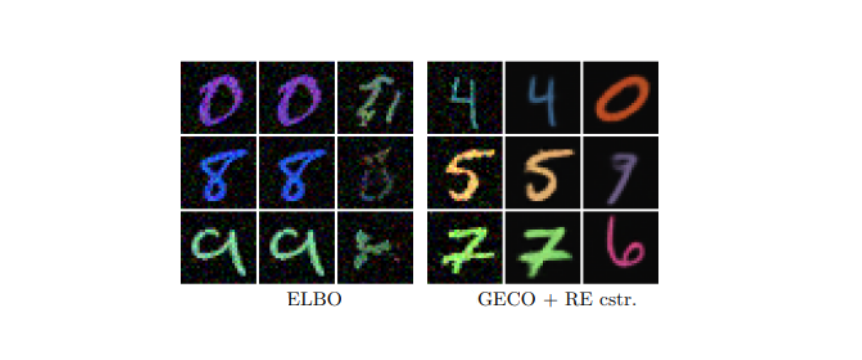
\includegraphics[width=\textwidth]{MNIST}
\caption{Note the differences in the last column of the ELBO dataset}
\centering
\end{figure}
\begin{figure}[t]
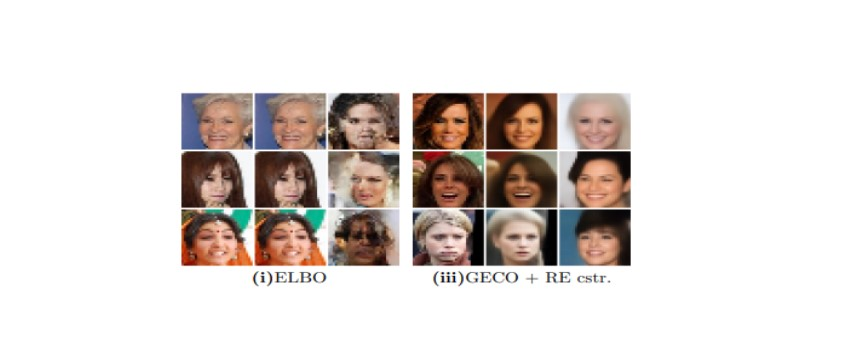
\includegraphics[width=\textwidth]{CelebA}
\caption{Note the differences in the last column of the ELBO dataset}
\centering
\end{figure}

	
\end{document}